\documentclass[tikz,border=4pt]{standalone}
\usepackage[T1]{fontenc}
\usepackage[utf8]{inputenc}
\usepackage{FiraSans}
\usepackage{amsmath}
\usetikzlibrary{arrows.meta,calc,positioning,decorations.pathreplacing}
\definecolor{ceBlue}{RGB}{42,96,153}
\definecolor{ceTeal}{RGB}{36,135,118}
\definecolor{ceGold}{RGB}{220,160,52}
\definecolor{ceRed}{RGB}{188,74,60}
\definecolor{ceInk}{RGB}{42,42,42}
\definecolor{ceGray}{RGB}{238,240,242}
\begin{document}
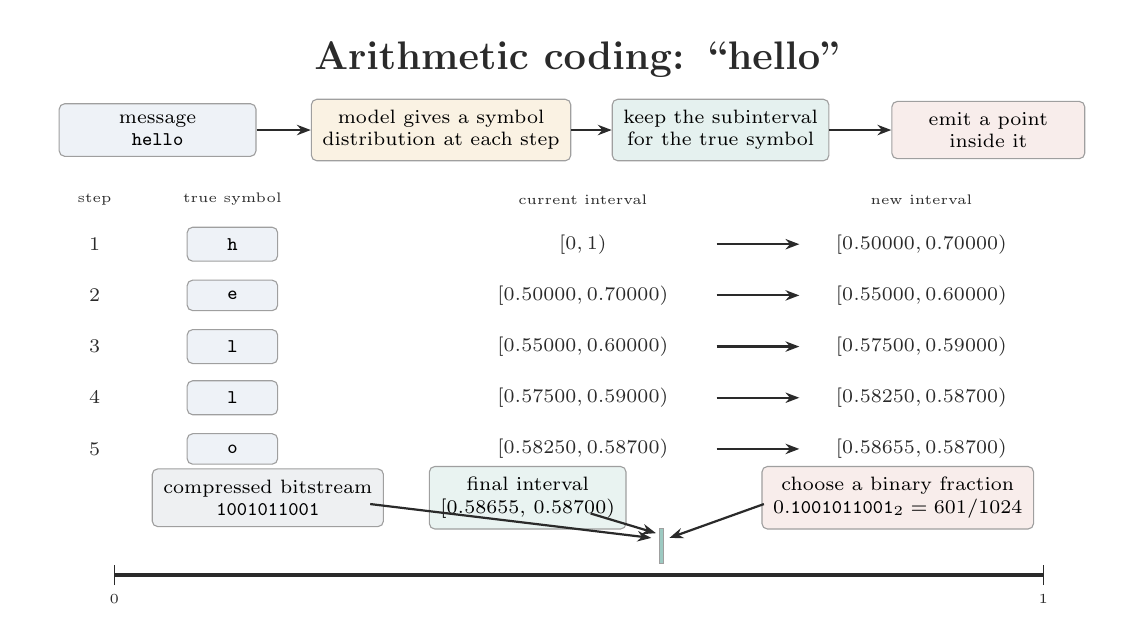
\begin{tikzpicture}[
  x=1cm,y=1cm,
  font=\sffamily,
  arr/.style={-{Stealth[length=5pt]}, thick, ceInk},
  lab/.style={font=\scriptsize, ceInk, align=center},
  tinylabel/.style={font=\tiny, ceInk, align=center},
  box/.style={draw=ceInk!45, rounded corners=2pt, fill=white, inner sep=4pt, font=\scriptsize, align=center},
]
  \path (-0.2,-0.75) rectangle (13.4,6.6);
  \node[font=\Large\bfseries, ceInk] at (6.8,6.2) {Arithmetic coding: ``hello''};

  \node[box, fill=ceBlue!8, minimum width=2.5cm] (msg) at (1.45,5.3) {message\\\texttt{hello}};
  \node[box, fill=ceGold!14, minimum width=3.1cm] (model) at (5.05,5.3) {model gives a symbol\\distribution at each step};
  \node[box, fill=ceTeal!12, minimum width=2.7cm] (interval) at (8.6,5.3) {keep the subinterval\\for the true symbol};
  \node[box, fill=ceRed!10, minimum width=2.45cm] (bits) at (12.0,5.3) {emit a point\\inside it};
  \draw[arr] (msg) -- (model);
  \draw[arr] (model) -- (interval);
  \draw[arr] (interval) -- (bits);

  \node[tinylabel] at (0.65,4.42) {step};
  \node[tinylabel] at (2.4,4.42) {true symbol};
  \node[tinylabel] at (6.85,4.42) {current interval};
  \node[tinylabel] at (11.15,4.42) {new interval};

  \foreach \i/\sym/\oldlo/\oldhi/\newlo/\newhi/\y in {
    1/h/0/1/0.50000/0.70000/3.85,
    2/e/0.50000/0.70000/0.55000/0.60000/3.20,
    3/l/0.55000/0.60000/0.57500/0.59000/2.55,
    4/l/0.57500/0.59000/0.58250/0.58700/1.90,
    5/o/0.58250/0.58700/0.58655/0.58700/1.25
  } {
    \node[lab] at (0.65,\y) {\i};
    \node[box, fill=ceBlue!8, minimum width=1.15cm] at (2.4,\y) {\texttt{\sym}};
    \node[lab] at (6.85,\y) {$[\oldlo,\oldhi)$};
    \node[lab] at (11.15,\y) {$[\newlo,\newhi)$};
    \draw[arr] (8.55,\y) -- (9.6,\y);
  }

  \draw[very thick, ceInk] (0.9,-0.35) -- (12.7,-0.35);
  \draw[ceInk] (0.9,-0.48) -- (0.9,-0.22);
  \draw[ceInk] (12.7,-0.48) -- (12.7,-0.22);
  \node[tinylabel] at (0.9,-0.65) {$0$};
  \node[tinylabel] at (12.7,-0.65) {$1$};

  \fill[ceTeal!45] (7.82,-0.2) rectangle (7.88,0.24);
  \draw[ceInk!45] (7.82,-0.2) rectangle (7.88,0.24);
  \node[box, fill=ceTeal!10] at (6.15,0.63) {final interval\\$[0.58655,\,0.58700)$};
  \draw[arr] (6.95,0.43) -- (7.78,0.18);

  \node[box, fill=ceRed!10, minimum width=3.4cm] at (10.85,0.63)
    {choose a binary fraction\\$0.\texttt{1001011001}_2 = 601/1024$};
  \draw[arr] (9.15,0.55) -- (7.95,0.12);
  \node[box, fill=ceGray, minimum width=2.5cm] at (2.85,0.63)
    {compressed bitstream\\\texttt{1001011001}};
  \draw[arr] (4.15,0.55) -- (7.72,0.12);
\end{tikzpicture}
\end{document}
